\documentclass[aspectratio=169,compress]{beamer}
\usepackage[T1]{fontenc}
\usepackage{lmodern}
\usepackage{graphicx}
\usepackage{xcolor}
\usepackage{etoolbox}
\usepackage{amsmath}

% Match the established FRIDA slide style.
\definecolor{NordBody}{HTML}{4C566A}
\definecolor{NordBlue}{HTML}{5E81AC}
\definecolor{NordPanel}{HTML}{ECEFF4}
\definecolor{NordRed}{HTML}{BF616A}

% Retain the custom FRIDA styling while adding Beamer's standard mini-frame
% section navigation.  Completed and current frames are filled; future frames
% remain hollow.  The cumulative-fill state follows the established etoolbox
% approach documented at https://tex.stackexchange.com/questions/61241/.
\useoutertheme[subsection=false]{miniframes}
\setbeamercolor{section in head/foot}{fg=NordBlue,bg=white}
\setbeamercolor{mini frame}{fg=NordBlue,bg=white}
\setbeamercolor{lower separation line head}{bg=NordPanel}
\setbeamerfont{section in head/foot}{size=\tiny}

\newif\ifnavbeforecurrent
\pretocmd\insertnavigation{\navbeforecurrenttrue}{}{}

\newcommand{\fridanavigationdot}{%
  \begin{pgfpicture}{0pt}{0pt}{0.1cm}{0.1cm}
    \pgfpathcircle{\pgfpoint{0.05cm}{0.05cm}}{0.05cm}
    \ifnavbeforecurrent
      \pgfusepath{fill,stroke}
    \else
      \pgfusepath{stroke}
    \fi
  \end{pgfpicture}%
}

\defbeamertemplate*{mini frame}{frida progress}{%
  \begin{pgfpicture}{0pt}{0pt}{0.1cm}{0.1cm}
    \pgfpathcircle{\pgfpoint{0.05cm}{0.05cm}}{0.05cm}
    \pgfusepath{fill,stroke}
  \end{pgfpicture}%
  \global\navbeforecurrentfalse
}
\defbeamertemplate*{mini frame in current section}{frida progress}{\fridanavigationdot}
\defbeamertemplate*{mini frame in current subsection}{frida progress}{\fridanavigationdot}
\defbeamertemplate*{mini frame in other section}{frida progress}{\fridanavigationdot}
\defbeamertemplate*{mini frame in other subsection}{frida progress}{\fridanavigationdot}
\setbeamertemplate{mini frame}[frida progress]
\setbeamertemplate{mini frame in current section}[frida progress]
\setbeamertemplate{mini frame in current subsection}[frida progress]
\setbeamertemplate{mini frame in other section}[frida progress]
\setbeamertemplate{mini frame in other subsection}[frida progress]

\setbeamertemplate{footline}{
  \hspace{1em}%
  \usebeamercolor[fg]{page number in head/foot}%
  \usebeamerfont{page number in head/foot}%
  \insertframenumber\,/\,\inserttotalframenumber%
  \vskip2pt%
}
\beamertemplatenavigationsymbolsempty
\setbeamerfont{frametitle}{size=\large}
\setbeamercolor{normal text}{fg=NordBody}
\setbeamercolor{title}{fg=NordBlue}
\setbeamercolor{frametitle}{fg=NordBlue}
\setbeamercolor{structure}{fg=NordBlue}
\setbeamercolor{itemize item}{fg=NordBlue}
\hypersetup{colorlinks=true,allcolors=NordBlue}

\newcommand{\plotframe}[2]{%
  \begin{frame}
    \frametitle{#1}
    \centering
    \includegraphics[width=0.985\linewidth,height=0.845\textheight,keepaspectratio]{#2}
  \end{frame}%
}

\newcommand{\chapterframe}[2]{%
  \begin{frame}
    \frametitle{#1}
    \vfill
    \begin{center}
      \begin{minipage}{0.84\linewidth}
        \raggedright
        \Large #2
      \end{minipage}
    \end{center}
    \vfill
  \end{frame}%
}

\title{FRIDA ADC Characterization}
\subtitle{From comparator choices to measured static linearity}
\author{Kennedy Caisley}
\institute{University of Bonn}
\date{12 August 2026}

\begin{document}

\begingroup
\setbeamertemplate{headline}{}
\begin{frame}
  \titlepage
  \vfill
  \begin{center}
    
\includegraphics[height=1.15cm]{../images/logo_bonn.jpg}%
    \hspace{0.75cm}%
    
\includegraphics[height=1.15cm]{../images/logo_ftd.jpg}%
    \hspace{0.75cm}%
    
\includegraphics[height=1.27cm]{../images/logo_silab.png}%
  \end{center}
\end{frame}

\begin{frame}
  \frametitle{One progressive characterization chain}
  \large
  \begin{enumerate}
    \item Bound comparator design trade-offs in SPICE, then measure the fabricated comparators.
    \item Measure the CDAC element weights which set the SAR decision levels.
    \item Establish comparator-to-logic timing before interpreting conversion results.
    \item Follow noise through rate, output-code, and bit-decision distributions, then quantify power.
    \item Close with a slow monotonic ramp: transfer, code density, DNL, and INL.
  \end{enumerate}
\end{frame}
\endgroup

\section[Background]{Detector and ADC background}
\chapterframe{Detector rates set the ADC target envelope}{%
  Fluence and pixel pitch establish the incoming hit rate.  The integration window and ADC resolution then set the maximum count rate, while the Murmann survey places the FRIDA design goal against published ADCs.}

\plotframe{Fluence and pixel pitch set the per-pixel hit rate}{../../phys/results/hit_rate_vs_fluence.pdf}
\plotframe{Integration time and resolution limit the counting rate}{../../phys/results/max_counting_rate_vs_window.pdf}

\plotframe{The design goal targets 11 ENOB at 10 MS/s}{../../phys/results/adc_survey_enob_vs_rate.pdf}
\plotframe{The resolution target sits in a compact-area regime}{../../phys/results/adc_survey_enob_vs_area.pdf}
\plotframe{The same target requires roughly 10 pJ per conversion}{../../phys/results/adc_survey_enob_vs_energy.pdf}
\plotframe{Area and conversion energy must be met together}{../../phys/results/adc_survey_energy_vs_area.pdf}
\plotframe{Walden FoM captures the combined efficiency target}{../../phys/results/adc_survey_fomw_vs_area.pdf}

\section[Design]{Comparator design}
\begin{frame}
  \frametitle{Comparator candidates: the design-space question}
  \centering
  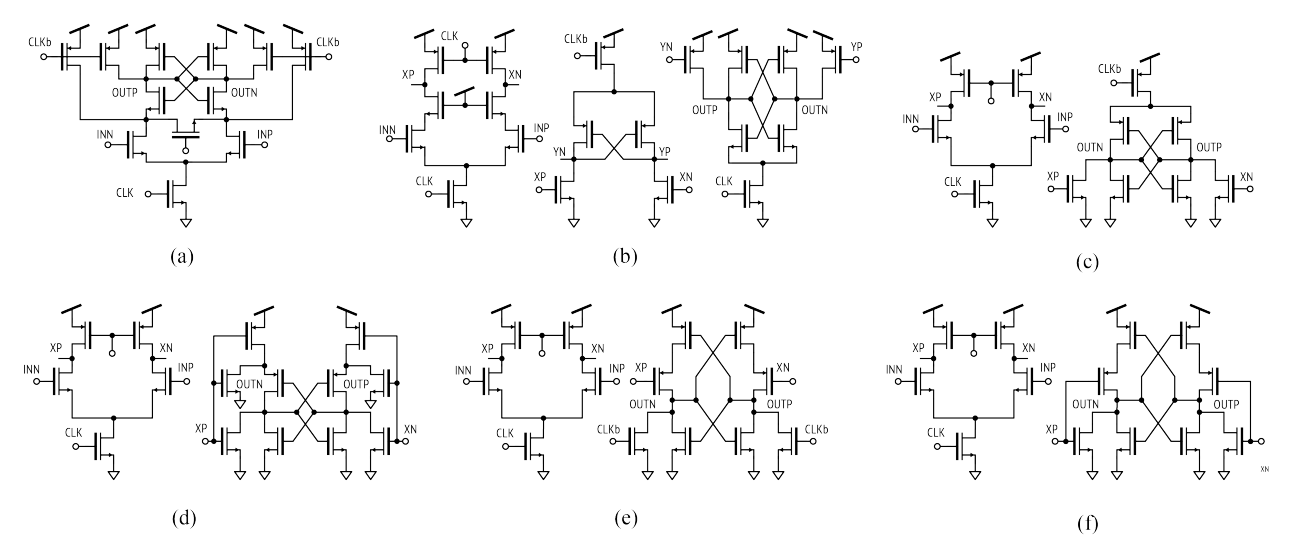
\includegraphics[width=0.93\linewidth,height=0.53\textheight,keepaspectratio]{../images/comparator_architectures.png}

  \vspace{-0.25em}
  {\tiny
    \href{https://www2.eecs.berkeley.edu/Pubs/TechRpts/2025/EECS-2025-21.pdf}{Liu, ``Automated and Process-Portable Generation of Data Converters,'' UCB/EECS-2025-21, 2025}
  }

  \vspace{0.55em}
  \begin{minipage}{0.89\linewidth}
    \small
    A 297-member HDL21/SPICE campaign varies topology and device size around the fabricated FRIDA comparator. Each candidate uses the same transient-noise S-curve bench and 30 ns metastability settling window.
  \end{minipage}
\end{frame}

\plotframe{Area exposes the complete noise, power, and timing landscape}{../../build/analysis/comp/20260812_0034/comp_candidate_noise_power_settling.pdf}
\plotframe{The fabricated comparator anchors the noise--power trade-off}{../../build/analysis/comp/20260812_0034/comp_candidate_noise_power_tradeoff.pdf}

\section[Comparators]{Comparator measurements}
\chapterframe{Fabricated comparators: does silicon support the model?}{%
  Full S-curves separate threshold from input-referred noise. Common-mode and track/hold campaigns reveal operating-envelope and sampling effects independently for ADC00--ADC03.}

\plotframe{ADC00 comparator across the qualified common-mode range}{../../build/analysis/comp/20260805_2213/adc00_comparator_common_mode.pdf}
\plotframe{ADC01 comparator across the qualified common-mode range}{../../build/analysis/comp/20260805_2213/adc01_comparator_common_mode.pdf}
\plotframe{ADC02 comparator across the qualified common-mode range}{../../build/analysis/comp/20260805_2213/adc02_comparator_common_mode.pdf}
\plotframe{ADC03 comparator across the qualified common-mode range}{../../build/analysis/comp/20260805_2213/adc03_comparator_common_mode.pdf}
\plotframe{ADC00 sampling: five complementary CDAC states}{../../build/analysis/comp/20260805_1931/adc00_comparator_sampling_noise.pdf}
\plotframe{ADC01 sampling: five complementary CDAC states}{../../build/analysis/comp/20260805_1931/adc01_comparator_sampling_noise.pdf}
\plotframe{ADC02 sampling: five complementary CDAC states}{../../build/analysis/comp/20260805_1931/adc02_comparator_sampling_noise.pdf}
\plotframe{ADC03 sampling: five complementary CDAC states}{../../build/analysis/comp/20260805_1931/adc03_comparator_sampling_noise.pdf}

\section[CDAC]{CDAC measurements}
\chapterframe{CDAC characterization: measure the SAR step sizes}{%
  A-to-B transition S-curves extract all P/N element weights in both directions and diffcap modes. These measured weights provide an independent digital decoding for the final ramp test.}

\plotframe{CDAC mismatch is similar in structure but channel-specific}{../../build/analysis/adc/20260807_1916/adc00_adc03_cdac_ab_comparison.pdf}
\plotframe{ADC00 measured CDAC element values}{../../build/analysis/adc/20260807_1916/adc00_cdac_ab_values.pdf}
\plotframe{ADC01 measured CDAC element values}{../../build/analysis/adc/20260807_1916/adc01_cdac_ab_values.pdf}
\plotframe{ADC02 measured CDAC element values}{../../build/analysis/adc/20260807_1916/adc02_cdac_ab_values.pdf}
\plotframe{ADC03 measured CDAC element values}{../../build/analysis/adc/20260807_1916/adc03_cdac_ab_values.pdf}

\section[Operation]{ADC operation}
\chapterframe{Comparator-to-logic offset: choose decision time, not just clock rate}{%
  Sweeping the logic edge around the comparator edge exposes the actual settling margin. The usable conversion-rate region is the one that remains quiet across timing offsets, not merely the fastest point that produces codes.}

\plotframe{ADC00 noise versus rate and comparator-to-logic offset}{../../build/analysis/adc/20260807_2351/adc00_noise_vs_conversion_rate_and_logic_offset.pdf}
\plotframe{ADC01 noise versus rate and comparator-to-logic offset}{../../build/analysis/adc/20260807_2351/adc01_noise_vs_conversion_rate_and_logic_offset.pdf}

\section[Speeds]{ADC at speeds}
\chapterframe{ADC at speed: when does noise begin to rise?}{%
  Fixed-input code spread is converted to input-referred noise and compared with generated and PEX SPICE where available. The rate sweep distinguishes the analog noise floor from timing-induced failures.}

\begin{frame}
  \frametitle{A 100 nF C6 sets the driver noise bandwidth}
  \begin{columns}[T,onlytextwidth]
    \begin{column}{0.58\textwidth}
      \footnotesize
      \setlength{\abovedisplayskip}{0.35em}
      \setlength{\belowdisplayskip}{0.35em}
      Unity gain uses $R_F=R_G=499~\Omega$.  For
      $R_\Sigma=R_{25}+R_{26}=998~\Omega$ and $C_6=100~\mathrm{nF}$,
      \[
        \begin{aligned}
          f_p&=\frac{1}{2\pi R_\Sigma C_6}=1.59~\mathrm{kHz},\\
          B_n&=\frac{\pi}{2}f_p=2.51~\mathrm{kHz}.
        \end{aligned}
      \]
      For $NG=1+R_F/R_G=2$, THS4541 datasheet Equation~6 is
      \[
        \begin{aligned}
          e_{no}^2={}&(e_{ni}NG)^2+2(i_nR_F)^2\\
                    &+2(4kTR_FNG).
        \end{aligned}
      \]
      At $T=300~\mathrm{K}$, with $e_{ni}=2.2~\mathrm{nV}/\sqrt{\mathrm{Hz}}$
      and $i_n=1.9~\mathrm{pA}/\sqrt{\mathrm{Hz}}$,
      \[
        \begin{aligned}
          e_{no}&=7.36~\mathrm{nV}/\sqrt{\mathrm{Hz}},\\
          v_{n,\mathrm{THS}}&=e_{no}\sqrt{B_n}
            =0.37~\mu\mathrm{V}_{\mathrm{RMS}}.
        \end{aligned}
      \]
      Adding $4kTR_\Sigma$ in RSS for the output resistors raises the ideal
      white-noise floor to $0.42~\mu\mathrm{V}_{\mathrm{RMS}}$.
    \end{column}
    \begin{column}{0.39\textwidth}
      \centering
      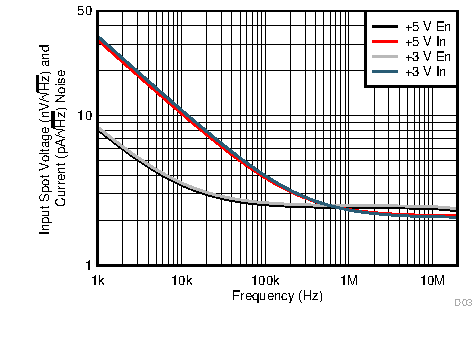
\includegraphics[width=\linewidth,height=0.52\textheight,keepaspectratio]{../images/ths4541_input_spot_noise.pdf}

      \scriptsize
      TI THS4541 datasheet, Figure 6-39

      \vspace{0.45em}
      \scriptsize
      The low-frequency rise, capacitor derating, ADC noise, drift, and
      instrument floor are excluded; $0.42~\mu\mathrm{V}_{\mathrm{RMS}}$ is a
      white-noise lower bound, not a predicted bench result.

      \vspace{0.35em}
      \href{https://www.ti.com/lit/gpn/ths4541}{Datasheet source: Figure 6-39 and Equation 6}
    \end{column}
  \end{columns}
\end{frame}

\plotframe{ADC00 input-referred noise versus conversion rate}{../../build/analysis/adc/20260808_0141/adc00_noise_vs_conversion_rate.pdf}
\plotframe{ADC01 input-referred noise versus conversion rate}{../../build/analysis/adc/20260808_0141/adc01_noise_vs_conversion_rate.pdf}

\section[Noise]{ADC noise analysis}
\chapterframe{Conversion paths: locate where output spread is created}{%
  Output distributions show the final code uncertainty. Bit-decision densities expose how the same uncertainty propagates through the SAR path and how it changes between 2 and 10 MS/s.}

\plotframe{ADC00 output codes at 50 mV}{../../build/analysis/adc/20260807_2343/adc00_50mv_dc_output_code_distributions.pdf}
\plotframe{ADC00 output-code violins at 50 mV}{../../build/analysis/adc/20260807_2343/adc00_50mv_dc_output_code_violins.pdf}
\plotframe{ADC00 decision paths at 50 mV and 2 MS/s}{../../build/analysis/adc/20260807_2343/adc00_50mv_2msps_decision_path_density.pdf}
\plotframe{ADC00 decision paths at 50 mV and 10 MS/s}{../../build/analysis/adc/20260807_2343/adc00_50mv_10msps_decision_path_density.pdf}
\plotframe{ADC01 output codes at 50 mV}{../../build/analysis/adc/20260807_2343/adc01_50mv_dc_output_code_distributions.pdf}
\plotframe{ADC01 output-code violins at 50 mV}{../../build/analysis/adc/20260807_2343/adc01_50mv_dc_output_code_violins.pdf}
\plotframe{ADC01 decision paths at 50 mV and 2 MS/s}{../../build/analysis/adc/20260807_2343/adc01_50mv_2msps_decision_path_density.pdf}
\plotframe{ADC01 decision paths at 50 mV and 10 MS/s}{../../build/analysis/adc/20260807_2343/adc01_50mv_10msps_decision_path_density.pdf}
\plotframe{ADC00 output codes at 100 mV}{../../build/analysis/adc/20260807_2343/adc00_100mv_dc_output_code_distributions.pdf}
\plotframe{ADC00 output-code violins at 100 mV}{../../build/analysis/adc/20260807_2343/adc00_100mv_dc_output_code_violins.pdf}
\plotframe{ADC00 decision paths at 100 mV and 2 MS/s}{../../build/analysis/adc/20260807_2343/adc00_100mv_2msps_decision_path_density.pdf}
\plotframe{ADC00 decision paths at 100 mV and 10 MS/s}{../../build/analysis/adc/20260807_2343/adc00_100mv_10msps_decision_path_density.pdf}
\plotframe{ADC01 output codes at 100 mV}{../../build/analysis/adc/20260807_2343/adc01_100mv_dc_output_code_distributions.pdf}
\plotframe{ADC01 output-code violins at 100 mV}{../../build/analysis/adc/20260807_2343/adc01_100mv_dc_output_code_violins.pdf}
\plotframe{ADC01 decision paths at 100 mV and 2 MS/s}{../../build/analysis/adc/20260807_2343/adc01_100mv_2msps_decision_path_density.pdf}
\plotframe{ADC01 decision paths at 100 mV and 10 MS/s}{../../build/analysis/adc/20260807_2343/adc01_100mv_10msps_decision_path_density.pdf}
\section[Power]{ADC power}
\plotframe{Whole-chip power rises with ADC00 conversion rate}{../../build/analysis/adc/20260818_0146/adc_power_vs_conversion_rate_adc00.pdf}
\plotframe{ADC01 confirms the same whole-chip power trend}{../../build/analysis/adc/20260818_0146/adc_power_vs_conversion_rate_adc01.pdf}
\plotframe{Ideal SPICE isolates one ADC macro across rate}{../../build/analysis/adc/20260818_0146/spice_ideal_power_vs_conversion_rate.pdf}
\plotframe{PEX increases the dynamic power of one ADC macro}{../../build/analysis/adc/20260818_0146/spice_pex_power_vs_conversion_rate.pdf}
\plotframe{Ideal SPICE locates power within one 100 ns conversion}{../../build/analysis/adc/20260818_0146/spice_ideal_10msps_supply_power.pdf}
\plotframe{PEX exposes rail-specific switching peaks}{../../build/analysis/adc/20260818_0146/spice_pex_10msps_supply_power.pdf}

\section[Linearity]{ADC linearity}
\plotframe{ADC00 slow-ramp transfer}{../../build/analysis/adc/20260812_1238/adc00_ramp_transfer.pdf}
\plotframe{ADC00 code-density histogram}{../../build/analysis/adc/20260812_1238/adc00_ramp_histogram.pdf}
\begin{frame}
  \frametitle{A-state sets direction; BOUT selects the P/N endpoint}
  \footnotesize
  Each A-to-B curve first gives a comparator-offset-corrected step:
  \[
    s_{q,i,d}=\operatorname{sign}(q)\operatorname{sign}(d)
    \frac{V_{\mathrm{off}}-V_{50,q,i,d}}{V_{\mathrm{DD,DAC}}}.
  \]
  A-state selects the direction of any change on side $q$:
  \[
    d_{q,i}=\begin{cases}0\!\rightarrow\!1,&A_{q,i}=0\\1\!\rightarrow\!0,&A_{q,i}=1,\end{cases}
    \qquad p_i=s_{P,i,d_{P,i}},\quad n_i=s_{N,i,d_{N,i}}.
  \]
  The SAR logic then sets $P_{\rm final}=1-B_i$ and $N_{\rm final}=B_i$.
  For equal P/N A-states:
  \[
    \begin{array}{c|cc}
      & B_i=0 & B_i=1\\ \hline
      A_i=0 & \text{raise P} & \text{raise N}\\
      A_i=1 & \text{drop N} & \text{drop P}
    \end{array}
  \]
  Thus $B_i$ selects an endpoint, not a fixed plate to move. Their separation
  is $w_i=p_i+n_i$. With fitted terminal weight
  $u=(w_{\rm ideal}\!\cdot w)/(w_{\rm ideal}\!\cdot w_{\rm ideal})$,
  \[
    D_{\mathrm{cal}}=\operatorname{round}\!\left[
      4095\,\frac{\sum_i B_iw_i+B_Tu}{\sum_i w_i+u}\right].
  \]
\end{frame}

\begin{frame}
  \frametitle{ADC00: extracted movements retain P/N and direction information}
  \centering
  \scriptsize
  P and N are normalized steps in $10^{-3}V_{\mathrm{DD,DAC}}$; $w$ is the
  final 4095-normalized decision weight.

  \vspace{0.45em}
  \setlength{\tabcolsep}{2.6pt}
  \renewcommand{\arraystretch}{0.82}
  \begin{tabular}{c c c r r r r@{\qquad}c c c r r r r}
    \hline
    Cap & A & dir. & ideal & P & N & $w$ & Cap & A & dir. & ideal & P & N & $w$ \\
    \hline
    C0 & 0 & 0--1 & 1536 & 156.305 & 149.903 & 1556.219 & C8 & 0 & 0--1 & 24 & 2.429 & 2.305 & 24.058 \\
    C1 & 1 & 1--0 & 1024 & 98.898 & 104.151 & 1031.941 & C9 & 1 & 1--0 & 20 & 1.775 & 2.045 & 19.410 \\
    C2 & 0 & 0--1 & 640 & 65.826 & 60.422 & 641.624 & C10 & 0 & 0--1 & 10 & 1.057 & 0.982 & 10.364 \\
    C3 & 1 & 1--0 & 384 & 35.276 & 39.855 & 381.834 & C11 & 1 & 1--0 & 8 & 0.762 & 1.023 & 9.073 \\
    C4 & 0 & 0--1 & 192 & 18.579 & 16.359 & 177.562 & C12 & 0 & 0--1 & 8 & 0.807 & 0.752 & 7.923 \\
    C5 & 1 & 1--0 & 128 & 10.093 & 12.321 & 113.911 & C13 & 1 & 1--0 & 4 & 0.260 & 0.449 & 3.607 \\
    C6 & 0 & 0--1 & 64 & 6.208 & 6.305 & 63.598 & C14 & 0 & 0--1 & 2 & 0.337 & 0.199 & 2.723 \\
    C7 & 1 & 1--0 & 48 & 4.626 & 4.694 & 47.364 & C15 & 1 & 1--0 & 2 & 0.188 & 0.359 & 2.781 \\
    \hline
  \end{tabular}

  \vspace{0.65em}
  \footnotesize Terminal weight: 1.009 LSB. All 17 normalized weights sum to 4095 exactly.
\end{frame}

\plotframe{ADC00 measured weights depart from the ideal at several redundant bits}{../../build/analysis/adc/20260812_1238/adc00_ramp_weights.pdf}
\plotframe{Direction matching is physical, but does not transfer into lower INL}{../../build/analysis/adc/20260812_1238/adc00_ramp_nonlinearity.pdf}
\plotframe{ADC01 slow-ramp transfer}{../../build/analysis/adc/20260812_1238/adc01_ramp_transfer.pdf}
\plotframe{ADC01 code-density histogram}{../../build/analysis/adc/20260812_1238/adc01_ramp_histogram.pdf}
\plotframe{ADC01 DNL and INL}{../../build/analysis/adc/20260812_1238/adc01_ramp_nonlinearity.pdf}
\plotframe{ADC02 slow-ramp transfer}{../../build/analysis/adc/20260812_1238/adc02_ramp_transfer.pdf}
\plotframe{ADC02 code-density histogram}{../../build/analysis/adc/20260812_1238/adc02_ramp_histogram.pdf}
\plotframe{ADC02 DNL and INL}{../../build/analysis/adc/20260812_1238/adc02_ramp_nonlinearity.pdf}
\plotframe{ADC03 slow-ramp transfer}{../../build/analysis/adc/20260812_1238/adc03_ramp_transfer.pdf}
\plotframe{ADC03 code-density histogram}{../../build/analysis/adc/20260812_1238/adc03_ramp_histogram.pdf}
\plotframe{ADC03 DNL and INL}{../../build/analysis/adc/20260812_1238/adc03_ramp_nonlinearity.pdf}

\end{document}
